%%%%%%%%%%%%%%%%%%%%% file typeinst.tex %%%%%%%%%%%%%%%%%%%%%%%%%
%
% This is the LaTeX source for the instructions to authors using
% the LaTeX document class 'llncs.cls' for contributions to
% the Lecture Notes in Computer Sciences series.
% http://www.springer.com/lncs       Springer Heidelberg 2006/05/04
%
% It may be used as a template for your own input - copy it
% to a new file with a new name and use it as the basis
% for your article.
%
% NB: the document class 'llncs' has its own and detailed documentation, see
% ftp://ftp.springer.de/data/pubftp/pub/tex/latex/llncs/latex2e/llncsdoc.pdf
%
%%%%%%%%%%%%%%%%%%%%%%%%%%%%%%%%%%%%%%%%%%%%%%%%%%%%%%%%%%%%%%%%%%%


\documentclass[runningheads,a4paper]{llncs}

\usepackage{amssymb}
\setcounter{tocdepth}{3}
\usepackage{graphicx}

\usepackage{url}
\urldef{\mailsa}\path|{alfred.hofmann, ursula.barth, ingrid.haas, frank.holzwarth,|
\urldef{\mailsb}\path|anna.kramer, leonie.kunz, christine.reiss, nicole.sator,|
\urldef{\mailsc}\path|erika.siebert-cole, peter.strasser, lncs}@springer.com|    
\newcommand{\keywords}[1]{\par\addvspace\baselineskip
\noindent\keywordname\enspace\ignorespaces#1}

\begin{document}

\mainmatter  % start of an individual contribution

% first the title is needed
\title{\huge{BORG} \\ \small{The RoboCup@Home team of the University of Groningen} \\ \large{Team Description Paper} \\ 2013}

% a short form should be given in case it is too long for the running head
\titlerunning{BORG - Team Description Paper}

\author{    
    Tim van Elteren \and
    Paul Neculoiu \and
    Christof Oost \and
    Amirhosein Shantia \and
    Ron Snijders \and
    Egbert van der Wal \and
    Tijn van der Zant
}
%
\authorrunning{The RoboCup@Home team of the University of Groningen}
% (feature abused for this document to repeat the title also on left hand pages)

% the affiliations are given next; don't give your e-mail address
% unless you accept that it will be published
\institute{Faculty of Mathematics and Natural Sciences, University of Groningen \\
    Dept. of Artificial Intelligence \\
    Cognitive Robotics Laboratory \\
    Groningen, The Netherlands \\
\url{http://www.ai.rug.nl}}

%
% NB: a more complex sample for affiliations and the mapping to the
% corresponding authors can be found in the file "llncs.dem"
% (search for the string "\mainmatter" where a contribution starts).
% "llncs.dem" accompanies the document class "llncs.cls".
%

\toctitle{BORG - Team Description Paper}
\tocauthor{BORG - The Robocup@Home team of the University of Groningen}
\maketitle

\begin{abstract}
This paper provides a description of the BORG team's robotic platform for the competition in the RoboCup@Home league. 
The robot is being developed at the Artificial Intelligence department of the University of Groningen, The Netherlands. 
The aim of the current design is to perform general service robot tasks as required by the @Home league of the RoboCup initiative utilizing mainly commercially available hardware components, open source libraries and a framework developed at the Cognitive Robotics Laboratory at the University of Groningen. 
An overview of the hardware and software specifications is given, with emphasis on the architecture and the methods currently being developed to address regular issues found in today's robotics such as navigation, recognition, manipulation and interaction.

\keywords{Robocup, Robocup@Home, Robotics, Domestic environments, Human Robot Interaction}
\end{abstract}

\section{Introduction}

The BORG team resides at the Artificial Intelligence department in the faculty of Mathematics and Natural Sciences at the University of Groningen, The Netherlands. 
The BORG is one of the first Dutch teams in the RoboCup@Home league.

Our current team consists of approximately 10-20 students and faculty members from the department of Artificial Intelligence and Computer Science. 
The BORG team is named after the small castles typically built on the hills that surround the Groningen province.

Accomplishing the tasks specified for the RoboCup@Home competition requires the students to be trained in pattern recognition on sensor data, human-robot interaction, actuators control, machine learning, reasoning and language processing. 
We use development techniques from eXtreme Programming such as unit-testing and agile design. 
The robot niche is defined as a stereotypical ``home'' environment for humans. 
Our approach towards autonomy is to combine a Pioneer robot platform with a humanoid Nao robot sitting on top of it.

This is an excellent combination for a platform where we can do what we are good at: developing Artificial Intelligence software. 
Nevertheless, the most important aspect of the project is that we do it because it is fun to do!

\section{Robot platform}
\subsection{Hardware architecture}

We aim to keep on improving our hardware architecture annually.
Our previous and current prototype of the robot is shown in figure \ref{fig:prototype}.
Our current hardware design provides us with higher load capacity and improved movability.

Like our previous design in 2011, our current design combines a Nao humanoid robot (from Aldebaran) sitting on top of a Pioneer 2 mobile platform (from Activmedia Robotics).
The purpose of using a Nao robot is to promote a natural human-machine interaction; whereas the Pioneer platform is intended to provide the robot an appropriate speed and a robust interaction with the environment.

In addition to sensors provided by the Nao and Pioneer 2, the platform has been extended with a rich set of additional sensors.
This includes two normal HD cameras, a directional microphone, two Kinect (for Xbox 360) cameras, one XTion PRO LIVE camera and one Laser Range Finder.
These additional sensors allows us to accomplish improved performance in object recognition, human robot interaction, manipulation, gesture recognition and navigation.

Extra processing power is provided by the use of additional laptops located just underneath the Nao robot.
These laptops and all other systems are interconnected using a local TCP/IP network.

Our current plans for improving the hardware platform, is the design and fabrication of a simple, yet powerful, robotic arm. 
This will allow us to manipulate heavy objects from a greater distance more easily than is currently possible using the Nao robot.

\begin{figure}
\centering
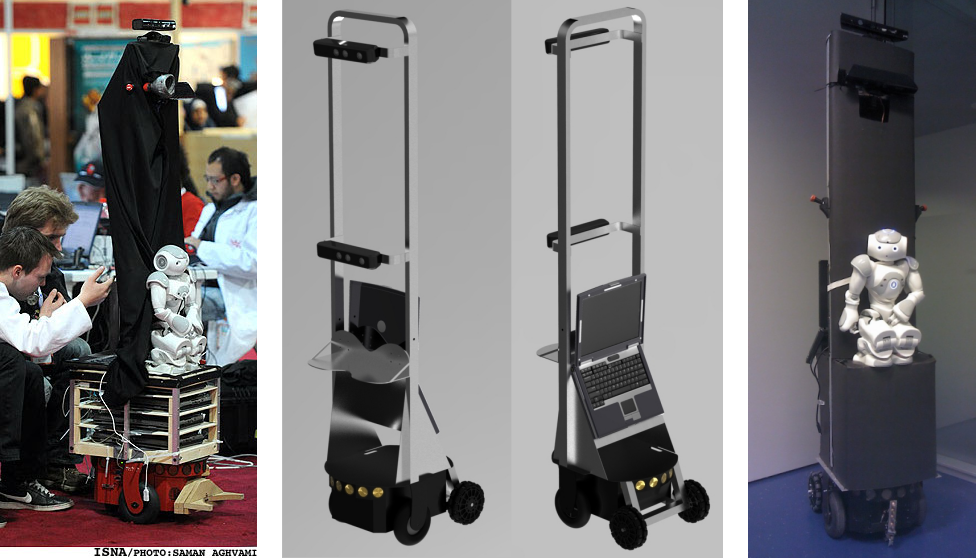
\includegraphics[width=0.9\textwidth]{figures/robot.png}
\caption{(\emph{Left}) Our previous prototype at the Iran Open 2011 competitions, a combination of a Nao and a Pioneer robot. (\emph{Middle}) Our current prototype design with additional omni wheels for higher load capacity. (\emph{Right}) Our current prototype as used in the Dutch Open 2012 competitions.}
\label{fig:prototype}
\end{figure}

\subsection{Software architecture}

The software architecture consists of sensor modules providing data about the world, and behavior modules that use this data to perform actions in the world. 
A separate navigation module uses the sensor information to estimate our location and orientation, and builds up a topological map to be able to reach 
previously visited destinations. 

The sensor modules run in parallel to each other. 
There is not one system for each modality: there might be multiple vision systems for instance. 
Some vision systems might specialize. 
For instance a module could only recognize faces.
However there can also be multiple systems that recognize 
the same category of objects: in this case, detections from multiple systems can be combined to increase reliability. 

We reuse existing and freely available software as much as possible. 
For vision, we use the OpenCV library\footnote{OpenCV is available from \url{http://opencv.willowgarage.com/wiki/}} \cite{bradski2008}. 
The `libfreenect'\footnote{libfreenect is available from \url{http://openkinect.org/wiki/Main_Page}} and 'openni'\footnote{openni is available from \url{http://openni.org/}} libraries are used to interface with the Kinect sensor unit.
For machine learning we use the `pyBrain'\footnote{pyBrain is available from \url{http://pybrain.org}}, 
`pyFLANN'\footnote{pyFLANN is available from \url{http://www.cs.ubc.ca/~mariusm/index.php/FLANN/FLANN}}, 
and `pyFANN'\footnote{pyFANN is available from \url{http://leenissen.dk/fann/wp/}} libraries.

Furthermore, our own custom made software framework is compitable with ROS\footnote{ROS (Robot Operating System) is available from \url{http://www.ros.org}.}. This enables us to use third party software components and algorithms, such as AMCL\cite{fox2001kld} and GMapping\cite{grisetti2007improved} for navigation, more easily. 

\section{Focus of research interests}

\subsection{Grid Occupancy and Vision based navigation system}
%TODO: references?

The navigation module of our team is now mainly based on grid occupancy methods. 
The main problem addressed by occupancy grid mapping the problem of generating a consistent metric map from noisy or incomplete sensor data with additional knowledge of robot pose. 
Even with all these information it is sometimes difficult to say whether a place in the environment is occupied or not, because of ambiguities in the sensor data. 
Occupancy grid maps solve such problems by generating probabilistic grid maps. 
These grid maps are usually two-dimensional but nowadays with use of time of flight camera and rotation 2D lasers, 3D grids are also popular. 
The standard occupancy grid mapping algorithm is a version of Bayes filters, just like any other major mapping algorithm \cite{thrun2002robotic}\cite{elfes1989occupancy}

In addition to the popular gird based method, we do research on additional vision based navigation systems.
In our visual method, the robot brain organizes a set of visual keywords that describe the robot's perception of the environment similar to that of human topological navigation. 
The results of its experiences are processed by a model that finds cause and effect relationships between executed actions and changes in the environment. 
This allows the robot to learn from the consequences of its actions in the real world. 
The robot is resistant to non-major changes in the environment during training and testing phases. 
More specific, the robot takes several pictures from the environment with an RGB camera during the training phase. 
The raw images will be processed using the histogram of oriented gradients method (HoG) to extract salient edges in major directions. 
By using clustering on HoG results, similar scenes will be clustered based on visual appearances. 
Furthermore, a world model is made from the observations and actions taken during training. 
Finally, during testing, the robot selects actions that maximize the probability to reach its goal using model-based reinforcement learning algorithms \cite{hognav}.

\subsection{Online behavior learning}
\label{sec:online_bahavior}

Our behavior modules don't have a strong central controller. 
Behaviors applicable in a certain context are executed. 
In each of the tests at the competition, a different suite of behaviors and preconditions will be used to ensure a proper behavior for a specific context. 
There might be different implementations of the same behavior, so different methods to pick up an object might be implemented. 
The interval estimation algorithm \cite{Zant2005} (a machine learning system for real-time robotic learning) is used to select the best-performing implementation of a given behavior. 
This system is adaptive, so that if circumstances change other behaviors can be chosen. 
For example, grasping a bottle might use grasp behavior 1, but if the bottle is very different from the previously trained bottle, and it can't grasp it, it starts using the next best behavior.

If a behavior keeps failing, for example selecting similar behaviors with the same post-conditions but running out of time so it gets bored, then the behavior module raises a flag to the reasoning module which checks whether it has a general solution to the problem. 
An example of a general solution is to go back to the human and tell him/her which behavior failed.
This mechanism is integral in our architecture and should solve a lot of the problems of the GPSR test.

If the robot is in the 'playing' mode, the boredom still works, but then it starts adapting its behaviors if the set of implemented behaviors keep failing or only succeed partially, for example by the use of parameter tuning, reinforcement learning or genetic programming.

\subsection{Interactive scenario interpretation using scripts}

For the general purpose service robot challenge, we are working on a script-based system that tries to find suitable (sequences of) behaviors for a certain scenario. 
The scripts consists of other scripts and behaviors, with alternative actions.
These alternative actions are used to make the system more robust when getting unspecified, general or complex commands.
This architecture also allows for failures (like a lower level behavior that is not able to reach its goal) to be handled.

Dialogue with the user is used to gather more information about the scenario, and about the preferences the user has. 
The system can also learn new scripts, by letting a user explain the steps that a certain complex task consists of, in terms of actions that the system already has scripts or behaviors for. 
The robot then learns how to execute that task by creating a new script for it.

\subsection{Human detection, tracking and recognition}

Fast and reliable human detection, tracking and recognition has a crucial role during Human Robot Interaction (HRI).
For consistent interaction between the robot and humans, several communication modalities have to be perceived and acknowledged by both sides to ensure a smooth and noise-free exchange of information.

To satisfy these tasks, we perform human body and face detection through the use of various features such as SURF\cite{bay2008speeded}, SIFT\cite{yan1995sift}, edge-based shape descriptors or the Viola Jones face detector\cite{viola2001rapid}, color blob and motion detection. 
After initital detection of human using depth information, we initialize a bounding box on the back of the person in RGB image. 
Next, we use an advanced online tracking system which is based on a combination of a short FPS tracker, online model learner, and a template matcher (OpenTLD) \cite{kalal2010face}\cite{kalal2010forward}. 
A sample image of tracker can be seen in Figure \ref{fig:tld}.

We thus incrementally build a system where such modules are added sequentially in order of increasing complexity. 
The ``Follow Me'' test of the RoboCup@Home competition is a good benchmark to ensure a reliable system for use in unconstrained environments.
To ensure robustness we implement several of such under performing modules, which are not completely reliable used independently and then combine them in voting committees or cascade boosters to achieve a satisfactory enough performance, thus, when one such element performs sub-par, another can take its place and reduce the error.

Through the use of machine learning techniques, the HRI module is able to decide which of the modules is reliable or not and under what circumstances to include or discard certain modules and achieve the desired tasks.

\begin{figure}
\centering
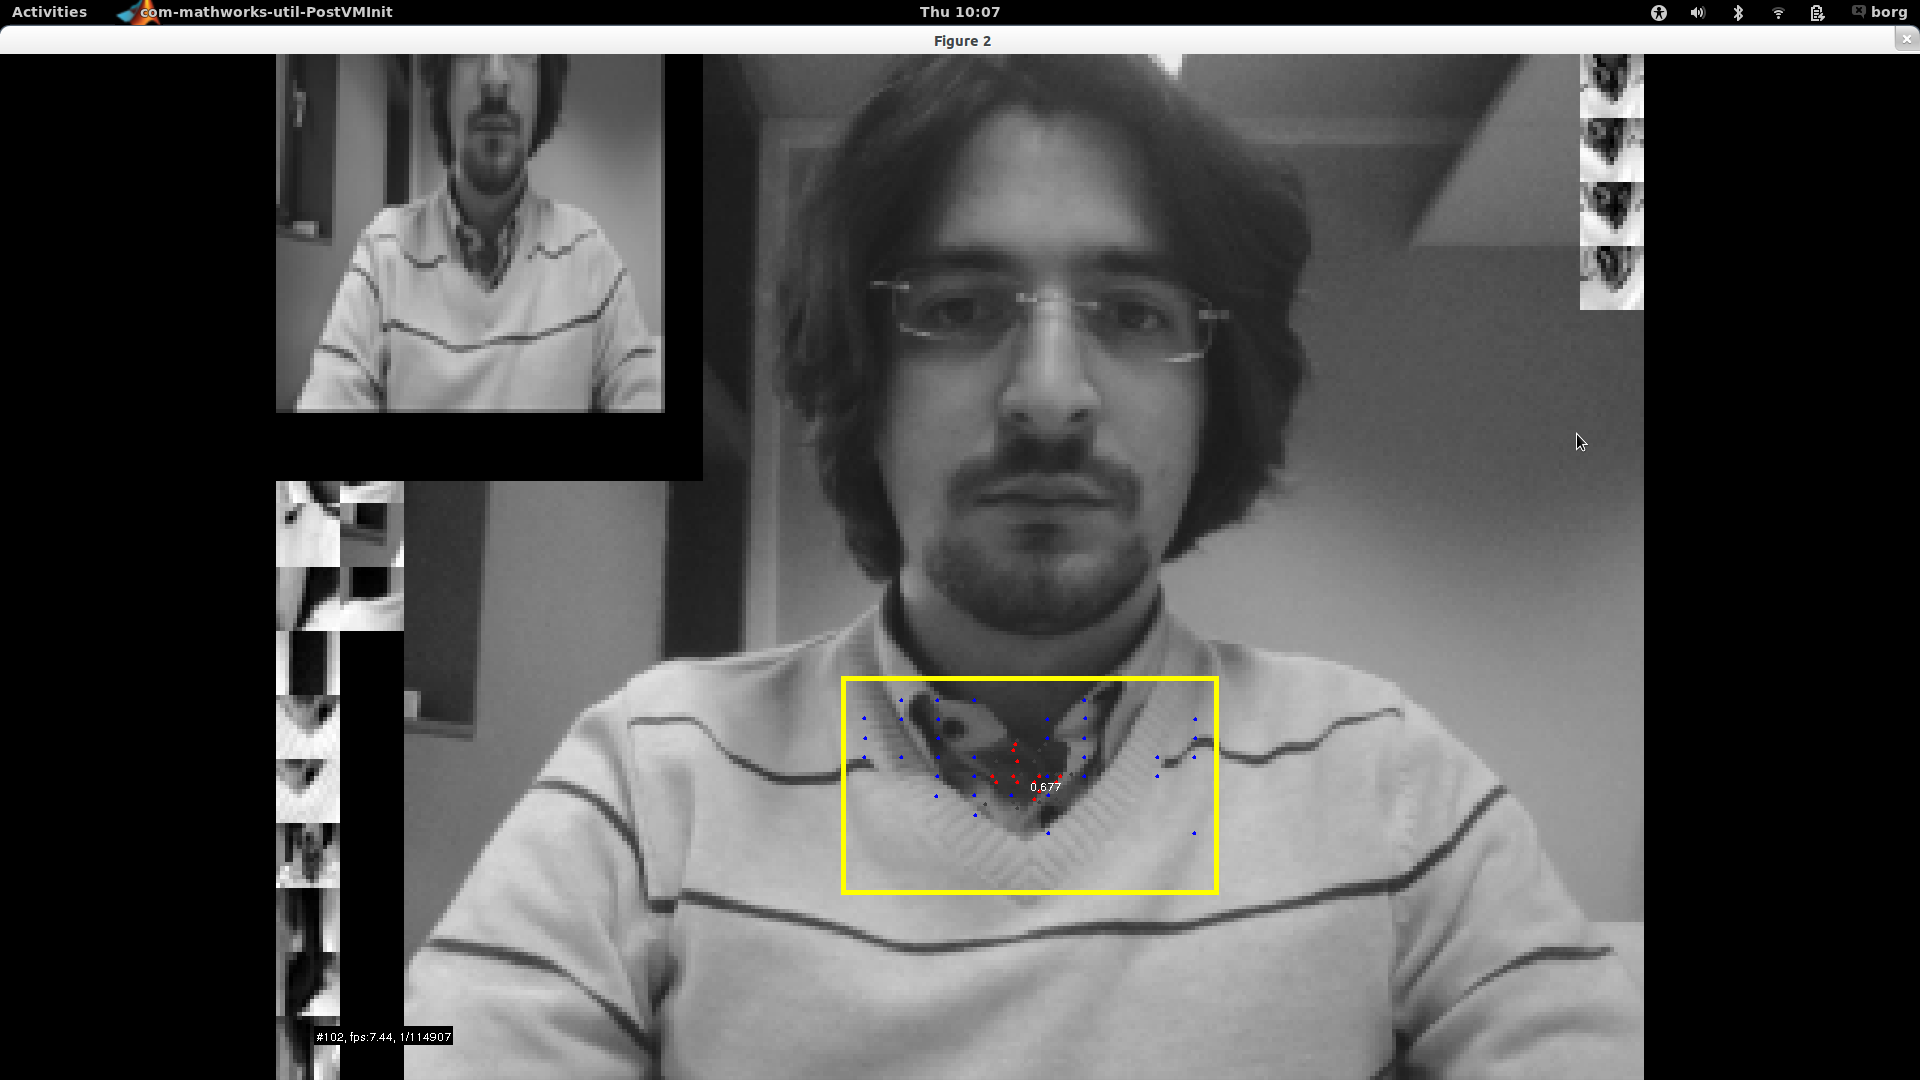
\includegraphics[width=0.7\textwidth]{figures/tld.png}
\caption{Sample image of the OpenTLD tracking system. The initial bounding box was automatically selected by depth processing. The system tracks and learns templates of the desired unknown object and the templates of the undesired locations.}
\label{fig:tld}
\end{figure}


\subsection{Learning to follow a person using reinforcement learning}

The aim of this project is to have a robot learn to follow a person rather than hard coding such a behavior. 
In our setup, the location of the person in the field of view of the robot and the distance to the person constitute the state space of the reinforcement learning problem.
Using Q-Learning \cite{watkins1992technical} the agent should find a mapping from these states to suitable acceleration speeds and turning angles. 
We will compare different grades of discretization for both state and action space to find the settings that will yield a good performance after a feasible learning time.

\subsection{Object Recognition and Manipulation}

With autonomous robots becoming more and more common, the interest in applications of mobile robotics increases. 
Many applications of robotics include the grasping and manipulation of objects. 
As many robotic manipulators have several degrees of freedom, controlling these manipulators is not a trivial task. 
The actuator needs to be guided along a proper trajectory towards the object to grasp, avoiding collisions with other objects and the surface supporting the object. 
In this project, the problem of learning a proper trajectory towards an object to grasp, located in front of a humanoid robot, the NAO from Aldebaran, is solved by using machine learning, and in particular a form of Reinforcement Learning (RL) tailored to continuous state and action spaces, the Continuous Actor Critic Learning Automaton (CACLA). 
Preliminary results show that even without initial training on demonstrations, the system is able to learn a proper trajectory by exploring the action space.
Current research focuses on shortening the training period by bootstrapping the actor on a set of recorded demonstrations where the actuators of the NAO were guided along a proper trajectory towards the object. 
By training the actor on these demonstrations, the initial estimates of the best action in each state is no longer random but already close to an optimal solution. 
By having the algorithm explore the space close to these trainings, it is able to optimize the actions it selects to come up with better solutions to the problem than demonstrated by the human. 


\subsection{Kinect and Xtion Pro Sensor Systems}

The depthsensor in the kinect and Xtion Pro sensor systems are used to gather depth information from a scene that enables the robot to gather more information from its surroundings than would be possible using only RGB cameras.

The depth information will be used for segmentation and 3D scene reconstruction for the use of navigation, thereby enabling obstacle avoidance and navigation using one of the freely available SLAM implementations provided by \url{OpenSLAM.org}.

Other uses include human-computer interaction (HCI), gesture recognition and training by example. 
The Kinect will also aid in the recognition of persons by their posture.

The libfreenect and OpenNI drivers are used to incorporate these sensors in our current Python software architecture.

\section{Relevance}

Our approach of combining a Nao and Pioneer to a new robot is easily reproducible, as it uses robots that are typically used for teaching purposes at universities.

Our setup allows to build a robot that exceeds the capabilities of both Nao and Pioneer alone without having to build a new robot from scratch.
Also with the Nao and Pioneer being widely used, both come with libraries (and other conveniences) which allows us to focus on the process of developing novel functionalities and behaviors.

Combining the Nao and the Pioneer integrates the best features of each robot into a more robust ``new robot'', which allows us to use the Nao's more fine-tuned movement to grab objects (and also gives the Nao a range of operation which is better suited to real world applications), while still being able to provide a speedy locomotion.
The additional HD cameras and the two Kinect cameras mounted at a height of approximately 180 cm allow for a good overview over real world scenery.

Apart from the hardware, our software architecture will make it possible for the robot to adapt its behavior to various environments, making it well suitable for applications outside ideal lab environments.


\section{Conclusion}
While still in the early stages of development, preliminary testing indicates that our platform can perform quite well in most, if not all, of the @Home challenges. 

The BORG team aims to explore the realm of general purpose service robotics for ongoing research work in human-robot interaction, computer vision, machine learning and control methods in ``real'', unconstrained environments.
The RoboCup@Home challenges are a fantastic benchmark to test these fields and the scientific validity of the systems presented above to cope with the challenges.

We hope that our main topics of investigation will bring fresh ideas and innovation into the world of service robotics.

\bibliographystyle{IEEEtran}
\bibliography{tdp}{}

\end{document}
